\chapter{Demostración práctica}
Para complementar el trabajo teórico, se incluye un archivo Jupyter Notebook con
implementaciones de juguete de ideas y algoritmos vistos (Ver \nameref{chap:tecnicas}).
Además, se utiliza el conocimiento adquirido en el trabajo anterior (\textit{Dashboards})
para generar datos de prueba y visualizarlos de manera interactiva utilizando \textit{Voila}.

\section{Distancia de Mahalanobis con distribuciones multivariantes}
Para esta demostración, se genera una distribución multivariante usando \\
\Verb#numpy.random.multivariate_normal# y haciendo que el umbral que define si un dato
es anómalo o no sea interactivo.

\noindent
\begin{minipage}{\linewidth}
	\centering
	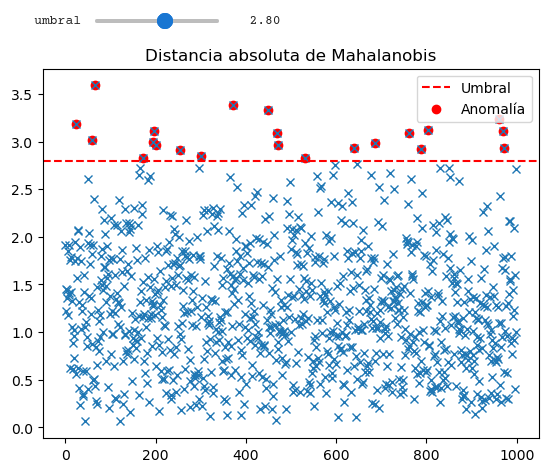
\includegraphics[width=\textwidth]{demo/mahalanobis_abs.png}
	\captionof{figure}{Plot de las muestras por distancia absoluta de Mahalanobis}\label{fig:demo11}
\end{minipage}

\noindent
\begin{minipage}{\linewidth}
	\centering
	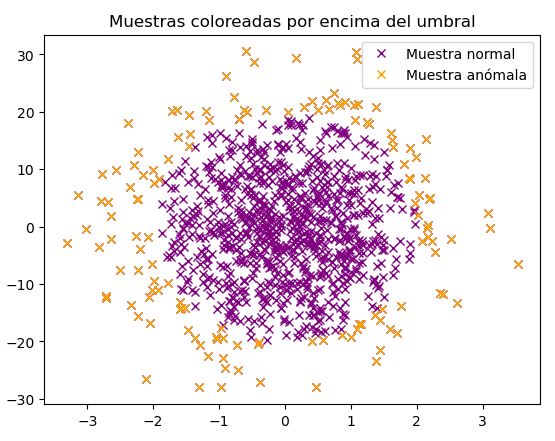
\includegraphics[width=\textwidth]{demo/mahalanobis_space.png}
	\captionof{figure}{Conjunto coloreado según la distancia de Mahalanobis}\label{fig:demo12}
\end{minipage}
\newpage{}
\section{Detección de anomalías basada en proximidad}
Para esta demostración, se utiliza la técnica de los $k$ vecinos más cercanos para detectar
anomalías. Se utiliza el mismo conjunto de datos que en la demostración anterior. En este caso,
tanto el número de vecinos $k$ como el umbral de anomalía son interactivos.

\noindent
\begin{minipage}{\linewidth}
	\centering
	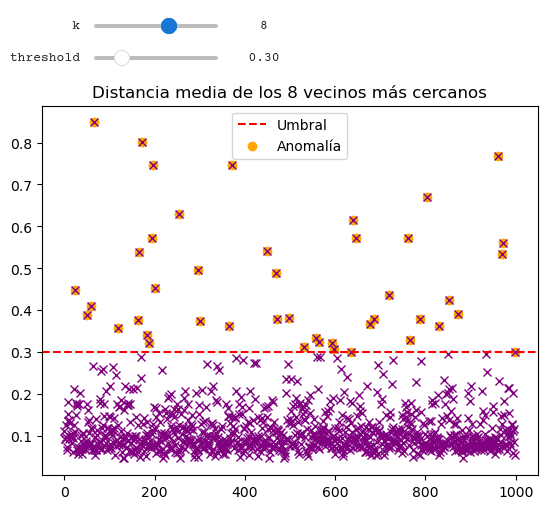
\includegraphics[width=\textwidth]{demo/knn_abs.png}
	\captionof{figure}{Plot de los datos por distancia media con los $k$ vecinos más cercanos}\label{fig:demo21}
\end{minipage}

Al contrario que con el metodo estadístico de Mahalanobis, se puede observar que se puede ajustar mucho más
fácilmente el umbral de anomalía con este método, ya que todos los valores cercanos a la media cuentan con una
distancia media con sus vecinos cercanos muy baja. Hay que tener en cuenta de que, como ya se ha comentado,
este es el caso para este conjunto de datos en concreto, pero no será así para todos los conjuntos que se observen.

La figura~\ref{fig:demo22} muestra el conjunto de datos coloreado en función de si es anómalo o no. En esta figura
se puede observar que, gracias al número $k$ de vecinos, no importa cómo de dispersos estén los datos respecto a
la media. Si se redujera $k$, habría menos datos considerados como anómalos debido a la naturaleza del conjunto.

\noindent
\begin{minipage}{\linewidth}
	\centering
	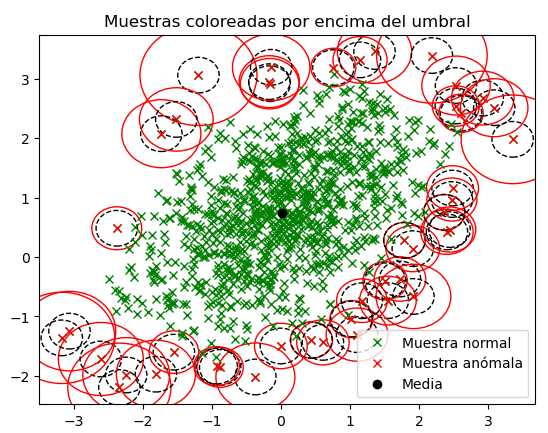
\includegraphics[width=\textwidth]{demo/knn_space.png}
	\captionof{figure}{Conjunto coloreado por anomalías con radios de distancia}\label{fig:demo22}
\end{minipage}

En la figura anterior, se puede observar que las muestras anómalas, marcadas con una cruz roja, cuentan con una
distancia con sus $k$ vecinos (círculos rojos) superior al umbral de anomalía (círculos negros). Si se aumentara
el umbral o se redujera el valor de $k$, muchas de dichas muestras no serían determinadas como ``anómalas''.
\newpage{}
\section{Clasificación con KNN y SVM}
En esta demostración, se juega con dos clasificadores diferentes:
\begin{itemize}
	\item Un clasificador de $k$ vecinos más cercanos (\textbf{KNN}) que requiere un umbral y un
		número $k$ de vecinos para clasificar las muestras.
	\item Un clasificador basado en densidad (\textbf{LOF}), que requiere un umbral para la
	clasificación.
\end{itemize}

Para el entreno, se utilizan los clasificadores de la librería \Verb#sklearn#. Todos los parámetros son interactivos.

\subsection{KNN}
\noindent
\begin{minipage}{\linewidth}
	\centering
	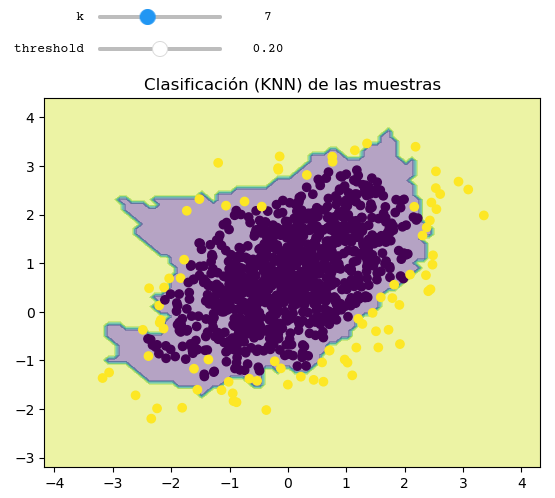
\includegraphics[width=\textwidth]{demo/knn.png}
	\captionof{figure}{Clasificación automática de las muestras por KNN}\label{fig:demo31}
\end{minipage}

\subsection{LOF}
\noindent
\begin{minipage}{\linewidth}
	\centering
	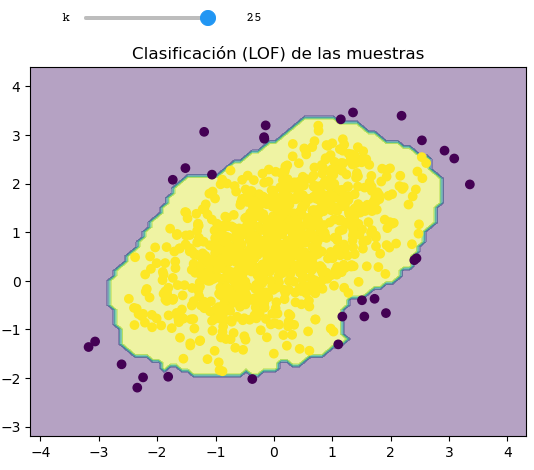
\includegraphics[width=\textwidth]{demo/lof.png}
	\captionof{figure}{Clasificación automática de las muestras por LOF}\label{fig:demo32}
\end{minipage}

Como se puede apreciar, el clasificador KNN es mucho más sensible a los cambios en los parámetros que el clasificador
LOF.~Además, al menos con este conjunto multivariante, el clasificador LOF es mucho más preciso, ya que no se basa
en un número de vecinos, sino en la densidad de los datos, lo que permite un mejor ajuste debido a la característica
del conjunto.
